\documentclass[12pt]{article}
\usepackage{graphicx}
%\documentclass[journal,12pt,twocolumn]{IEEEtran}
\usepackage[none]{hyphenat}
\usepackage{graphicx}
\usepackage{listings}
\usepackage[english]{babel}
\usepackage{graphicx}
\usepackage{caption}
\usepackage[parfill]{parskip}
\usepackage{hyperref}
\usepackage{booktabs}
%\usepackage{setspace}\doublespacing\pagestyle{plain}
\def\inputGnumericTable{}
\usepackage{color}                                            %%
    \usepackage{array}                                            %%
    \usepackage{longtable}                                        %%
    \usepackage{calc}                                             %%
    \usepackage{multirow}                                         %%
    \usepackage{hhline}                                           %%
    \usepackage{ifthen}
\usepackage{array}
\usepackage{amsmath}   % for having text in math mode
\usepackage{parallel,enumitem}
\usepackage{listings}
\lstset{
language=tex,
frame=single,
breaklines=true
}
%Following 2 lines were added to remove the blank page at the beginning
\usepackage{atbegshi}% http://ctan.org/pkg/atbegshi
\AtBeginDocument{\AtBeginShipoutNext{\AtBeginShipoutDiscard}}
%
%New macro definitions
\newcommand{\mydet}[1]{\ensuremath{\begin{vmatrix}#1\end{vmatrix}}}
\providecommand{\brak}[1]{\ensuremath{\left(#1\right)}}
\providecommand{\abs}[1]{\left\vert#1\right\vert}
\providecommand{\norm}[1]{\left\lVert#1\right\rVert}
\newcommand{\solution}{\noindent \textbf{Solution: }}
\newcommand{\myvec}[1]{\ensuremath{\begin{pmatrix}#1\end{pmatrix}}}
\let\vec\mathbf
\begin{document}
\begin{center}
\title{\textbf{Parallel Lines}}
\date{\vspace{-5ex}} %Not to print date automatically
\maketitle
\end{center}
\setcounter{page}{1}
\section*{11$^{th}$ Maths - Chapter 10}
This is Problem-3 from Exercise 10.4
\begin{enumerate}
\item Find the equations of the lines, which cut-off intercepts on the axes whose sum and product are 1 and -6,resspectively.
\section{Solution}
Let the x intercept be a and  the y intercept be b ,Then
\begin{align}
\myvec{a+b}&=1\label{1}\\
\myvec{ab}&=-6 \label{2}
\end{align}
upon simplifying \eqref{1} and \eqref{2}
\begin{align}
\myvec{a\\b}&=\myvec{3\\-2},\myvec{-2\\3}
\end{align}
Thus,the posiible equations of the line as
\begin{align}
\myvec{2,-3}\vec{x}&=6\\
\myvec{-3,2}\vec{x}&=6
\end{align}
\begin{figure}[h!]
\centering
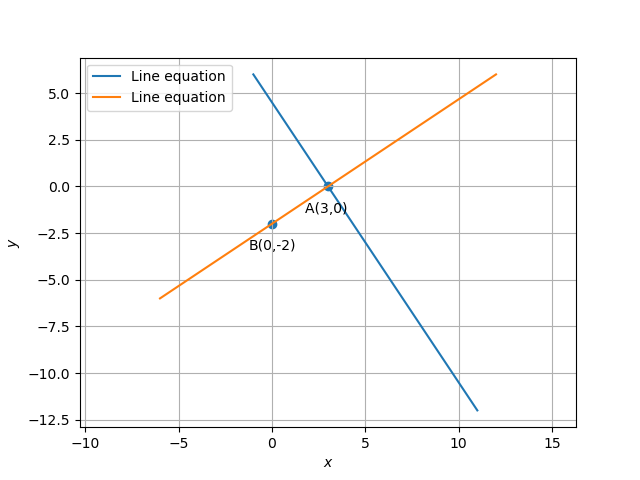
\includegraphics[width=\columnwidth]{./figs/inter.png}
\caption{}
\label{fig:inter.png}
\end{figure}
\end{enumerate}

\end{document}
